\chapter{Discussion}\label{ch:discussion}
In this chapter, we discuss our results after running the ABC-MCMC for our mutation model.

\section{Implementation}\label{sec:implementation}
All algorithms mentioned in this paper were implemented in Python 3.7.
To optimize the coalescent tree generation, repeat length determination, and likelihood determination processes, the
Numba package was used to compile and parallelize each function before running.
Simulations were run on the Cray supercomputer at the University of Hawaii at Manoa with $\texttt{cpus-per-task} = 20$
and $\texttt{mem}=10,000\texttt{MB}$.
All code (and this paper) can be found at the following Git repository:
\begin{equation*}
    \text{\href{https://github.com/glennga/micro-coa}{https://github.com/glennga/micro-coa}}
\end{equation*}

In this implementation, the following details differ from the descriptions laid in the previous chapters:
\begin{enumerate}
    \item The BFS we perform in~\autoref{subsec:coalescentRepeatLengthResolution} is not guaranteed to explore nodes
        of the same depth in a deterministic manner, but still performs a BFS nonetheless.
        Numba parallelizes this process, which leads to this randomness.
    \item In order to use~\autoref{alg:twoStageBackwardEvolution}, a common ancestor repeat length $\ell_1$ must be
        specified.
        \emph{We assume $\ell_1$ to be a nuisance parameter.}
        Given the variance associated with this process, we feel it is safe to assume this parameter does not need to be
        as precise as our other hyperparameters.
        We randomly select a repeat length from our observed data, and reduce the number of free parameters from
        four to three.
    \item In an effort to save space, two independent vectors $V$ and $E$ are not allocated for use at the same time
        in~\autoref{alg:twoStageBackwardEvolution}.
        Instead we define vector $V$ to hold the indices associated with each parent node to construct the edge set,
        and replace this with repeat lengths in the determination stage.
    \item The order with which the probabilities of some likelihood $\mathcal{\theta}$ are not guaranteed to be
        deterministic.
        Numba also parallelizes this process.
    \item In addition to recording the states required for Markov chain $X$ in~\autoref{alg:metropolis}, we also record
        the time between acceptances (known as the \emph{waiting time}), the likelihood of that point
        $\mathcal{L}(\theta^{(i)})$ (to avoid computing this later), the average distance associated with the generated
        data of the accepted parameter set and our observations, the time of acceptance in terms of iterations.
\end{enumerate}

\section{Hyperparameters}\label{sec:hyperparameters}
\begin{table}
    \begin{tabu} to \textwidth {|c|c|X|}
       \toprule
        Symbol & Value / Type & Detail / Explanation \\
        \hline
        $\kappa$ & 3 & Lower bound of our repeat length space $\mathbb{M}$. \\
        $\Omega$ & 30 & Upper bound of our repeat length space $\mathbb{M}$. \\
        $n$ & $100$ & Sample size, number of end individuals to simulate. \\
        $\tau_N(e)$ & $\exp\left(\sfrac{N}{\binom{\rho(e)}{2}}\right)$ & Generation determination function\\
        $N$ & $10,000$ & Effective population size. \\
        $\delta(e)$ & $\delta_A(e)$ & The distance function between two populations. \\
        $\epsilon$ & 0.55 & ABC cutoff to define approximate. \\
        $T_1$ & 100 & Number of simulations to run to determine $\Pr(\mathcal{M}(\theta) \approx \mathcal{D}_i)$. \\
        $\theta^{(1)}_c$ & 0.01 & Starting $c$ value for initial state of Markov chain $\theta^{(1)}$. \\
        $\theta^{(1)}_d$ & 0.001 & Starting $d$ value for initial state of Markov chain $\theta^{(1)}$ . \\
        $g_c(c)$ & $N(c, \sigma_c)$ & Proposal function to generate new $c$ values. \\
        $g_d(d)$ & $N(d, \sigma_d)$ & Proposal function to generate new $d$ values. \\
        $\sigma_c$ & 0.001 & Deviation associated with proposal function $g_c(c)$. \\
        $\sigma_d$ & 0.001 & Deviation associated with proposal function $g_d(d)$. \\
        $T_2$ & $55,000$ & Running time of Metropolis sampler. \\
        $b_c$ & $0.001$ & Bin size for $c$ histogram. \\
        $b_d$ & $0.0001$ & Bin size for $d$ histogram. \\
        $w_c(c)$ & $\Gamma(\ldots)$ & The assumed posterior distribution for $c$. \\
        $w_d(d)$ & $\Gamma(\ldots)$ & The assumed posterior distribution for $d$. \\
       \bottomrule
    \end{tabu}
    \caption{Table of our hyperparameters: their symbol, the value we chose, and a description of parameter itself.
    }\label{tab:hyperparameters}
\end{table}

\begin{figure}[t]
    \centering{%from scipy.stats import beta, norm, gamma
%from numpy import linspace, average, std
%x = linspace(0.0, 0.06)
%beta_x = beta.pdf(x, 2.462049740861992, 29.502013726920467, 0.0005845381630033533, 0.20813302210781293)
%norm_x = norm.pdf(x, 0.016615628892405383, 0.009681441990708757)
%gamma_x = gamma.pdf(x, 2.7500499267384706, 0.0003644996765732702, 0.005909429918741313)
%beta_mean = beta.mean(2.462049740861992, 29.502013726920467, 0.0005845381630033533, 0.20813302210781293)
%norm_mean = norm.mean(0.016615628892405383, 0.009681441990708757)
%gamma_mean = gamma.mean(2.7500499267384706, 0.0003644996765732702, 0.005909429918741313)
%print(f'Beta Mean: {beta_mean}\nNorm Mean: {norm_mean}\nGamma Mean: {gamma_mean}\n')
%print(f'Average: {average([beta_mean, norm_mean, gamma_mean])}')
%print(f'STD: {std([beta_mean, norm_mean, gamma_mean])}')
%
%print('\\addplot [very thick, blue!50!black] coordinates {')
%for i in list(zip(x, beta_x)):
%    print(f'\t({i[0]}, {i[1]})')
%
%print('};')

\addplot [very thick,blue!50!black] coordinates {
    (0.0, 0.0)
    (0.0012244897959183673, 3.185370433486203)
    (0.0024489795918367346, 12.849116233840686)
    (0.003673469387755102, 22.68508457236311)
    (0.004897959183673469, 31.161253710289554)
    (0.006122448979591836, 37.81753339019626)
    (0.007346938775510204, 42.608051910362846)
    (0.00857142857142857, 45.673546807801884)
    (0.009795918367346938, 47.235848966364564)
    (0.011020408163265306, 47.543261462563336)
    (0.012244897959183673, 46.84128896346183)
    (0.01346938775510204, 45.357261275791295)
    (0.014693877551020407, 43.29296827259877)
    (0.015918367346938776, 40.822011769104705)
    (0.01714285714285714, 38.08992329390769)
    (0.01836734693877551, 35.215851622648394)
    (0.019591836734693877, 32.29507317751616)
    (0.020816326530612245, 29.401856861684436)
    (0.022040816326530613, 26.59239242933872)
    (0.023265306122448978, 23.907606708272933)
    (0.024489795918367346, 21.375767433168306)
    (0.025714285714285714, 19.01482386260446)
    (0.02693877551020408, 16.834465434535016)
    (0.028163265306122447, 14.837900120588907)
    (0.029387755102040815, 13.023366635771918)
    (0.030612244897959183, 11.385401799256073)
    (0.03183673469387755, 9.91588787584037)
    (0.03306122448979592, 8.60490586919338)
    (0.03428571428571428, 7.4414203306201285)
    (0.03551020408163265, 6.413819877665804)
    (0.03673469387755102, 5.510335692046834)
    (0.037959183673469385, 4.71935806543318)
    (0.03918367346938775, 4.0296687732451515)
    (0.04040816326530612, 3.430604805269111)
    (0.04163265306122449, 2.912166846252753)
    (0.04285714285714286, 2.465083926187479)
    (0.044081632653061226, 2.080843872660651)
    (0.04530612244897959, 1.7516976048998794)
    (0.046530612244897955, 1.4706439089517072)
    (0.04775510204081632, 1.2314001171116706)
    (0.04897959183673469, 1.0283630694133308)
    (0.05020408163265306, 0.856563845615125)
    (0.05142857142857143, 0.7116190066923018)
    (0.052653061224489796, 0.5896804593163186)
    (0.05387755102040816, 0.48738553972437737)
    (0.055102040816326525, 0.40180849023321946)
    (0.05632653061224489, 0.3304141590851045)
    (0.05755102040816326, 0.2710144802527024)
    (0.05877551020408163, 0.22172807349347673)
    (0.06, 0.18094313682248273)
};
\node[black, above] at (axis cs:0.017,48){\small{$\hat{c} = 0.017$}};}
    \caption{Frequency surface of $c$ parameter.
    Our histogram was constructed using a bin size of $b_c = 0.001$
    In blue the least-squares estimate of a $\Gamma$ distribution for this histogram is displayed,
    with $a=3.740, \mathit{loc}=0.0009042, \mathit{scale}=0.003572$.
    }\label{fig:cData}
\end{figure}
\begin{figure}[t]
    \centering{\begin{tikzpicture}
    \begin{axis}[ymin=0,width=\linewidth, height=3.5cm, ylabel=$c$]

        \addplot+[very thick,green!50!black, mark=none] table[x=p, y=c] {trace1.dat};
        \addplot+[very thick,blue!50!black, mark=none] table[x=p, y=c] {trace2.dat};
        \addplot+[very thick,orange!50!black, mark=none] table[x=p, y=c] {trace3.dat};

    \end{axis}
\end{tikzpicture}}
    \caption{Trace plot of $c$ for all three runs of the Metropolis sampler.
    }\label{fig:cTrace}
\end{figure}

\begin{figure}[t]
    \centering{\pgfplotsset{compat=1.5}

%>>> x = linspace(0.0, 0.06)
%>>> beta_x = beta.pdf(x, 2.462049740861992, 29.502013726920467, 0.0005845381630033533, 0.20813302210781293)
%>>> norm_x = norm.pdf(x, 0.016615628892405383, 0.009681441990708757)
%>>> gamma_x = gamma.pdf(x, 2.7500499267384706, 0.0003644996765732702, 0.005909429918741313)
%>>> for i in list(zip(x, beta_x)):
%...     print(f'({i[0]}, {i[1]})')

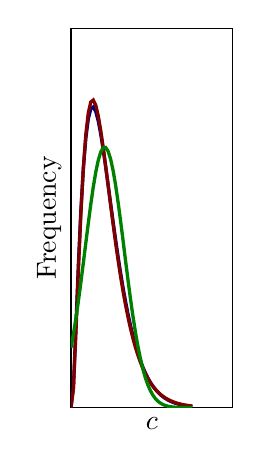
\begin{tikzpicture}
    \begin{axis}[
    width=0.3\linewidth, height=6.4cm,
    ylabel={Frequency}, ymax=60,
    xlabel={$c$}, xmin=0, xmax=0.08,
    samples=100, no markers, enlargelimits=false, legend style={at={(0.5,-0.35)},anchor=north},
    domain=0:1, ticks=none
    ]
    \addplot [very thick,blue!50!black] coordinates {
        (0.0, 0.0)
        (0.0012244897959183673, 3.185370433486203)
        (0.0024489795918367346, 12.849116233840686)
        (0.003673469387755102, 22.68508457236311)
        (0.004897959183673469, 31.161253710289554)
        (0.006122448979591836, 37.81753339019626)
        (0.007346938775510204, 42.608051910362846)
        (0.00857142857142857, 45.673546807801884)
        (0.009795918367346938, 47.235848966364564)
        (0.011020408163265306, 47.543261462563336)
        (0.012244897959183673, 46.84128896346183)
        (0.01346938775510204, 45.357261275791295)
        (0.014693877551020407, 43.29296827259877)
        (0.015918367346938776, 40.822011769104705)
        (0.01714285714285714, 38.08992329390769)
        (0.01836734693877551, 35.215851622648394)
        (0.019591836734693877, 32.29507317751616)
        (0.020816326530612245, 29.401856861684436)
        (0.022040816326530613, 26.59239242933872)
        (0.023265306122448978, 23.907606708272933)
        (0.024489795918367346, 21.375767433168306)
        (0.025714285714285714, 19.01482386260446)
        (0.02693877551020408, 16.834465434535016)
        (0.028163265306122447, 14.837900120588907)
        (0.029387755102040815, 13.023366635771918)
        (0.030612244897959183, 11.385401799256073)
        (0.03183673469387755, 9.91588787584037)
        (0.03306122448979592, 8.60490586919338)
        (0.03428571428571428, 7.4414203306201285)
        (0.03551020408163265, 6.413819877665804)
        (0.03673469387755102, 5.510335692046834)
        (0.037959183673469385, 4.71935806543318)
        (0.03918367346938775, 4.0296687732451515)
        (0.04040816326530612, 3.430604805269111)
        (0.04163265306122449, 2.912166846252753)
        (0.04285714285714286, 2.465083926187479)
        (0.044081632653061226, 2.080843872660651)
        (0.04530612244897959, 1.7516976048998794)
        (0.046530612244897955, 1.4706439089517072)
        (0.04775510204081632, 1.2314001171116706)
        (0.04897959183673469, 1.0283630694133308)
        (0.05020408163265306, 0.856563845615125)
        (0.05142857142857143, 0.7116190066923018)
        (0.052653061224489796, 0.5896804593163186)
        (0.05387755102040816, 0.48738553972437737)
        (0.055102040816326525, 0.40180849023321946)
        (0.05632653061224489, 0.3304141590851045)
        (0.05755102040816326, 0.2710144802527024)
        (0.05877551020408163, 0.22172807349347673)
        (0.06, 0.18094313682248273)
    };
    \addplot [very thick,red!50!black] coordinates {
        (0.0, 0.0)
        (0.0012244897959183673, 3.118662230643064)
        (0.0024489795918367346, 11.936583901014794)
        (0.003673469387755102, 21.782941926087133)
        (0.004897959183673469, 30.720133265436072)
        (0.006122448979591836, 37.94504054139017)
        (0.007346938775510204, 43.2228187238339)
        (0.00857142857142857, 46.61549634979339)
        (0.009795918367346938, 48.33225099833951)
        (0.011020408163265306, 48.64332942364865)
        (0.012244897959183673, 47.830688483184105)
        (0.01346938775510204, 46.16075314068907)
        (0.014693877551020407, 43.870686496639365)
        (0.015918367346938776, 41.16286974330062)
        (0.01714285714285714, 38.20425079470016)
        (0.01836734693877551, 35.12843953857918)
        (0.019591836734693877, 32.03920702110401)
        (0.020816326530612245, 29.01455169992369)
        (0.022040816326530613, 26.110826153339044)
        (0.023265306122448978, 23.366632887210365)
        (0.024489795918367346, 20.80633690652475)
        (0.025714285714285714, 18.443130936544872)
        (0.02693877551020408, 16.281643533039265)
        (0.028163265306122447, 14.320112223137059)
        (0.029387755102040815, 12.552160994767766)
        (0.030612244897959183, 10.968229142562846)
        (0.03183673469387755, 9.556700224661178)
        (0.03306122448979592, 8.304778068511268)
        (0.03428571428571428, 7.199152965966464)
        (0.03551020408163265, 6.226496451572009)
        (0.03673469387755102, 5.373818020485163)
        (0.037959183673469385, 4.628712216538371)
        (0.03918367346938775, 3.9795199378110513)
        (0.04040816326530612, 3.4154236846611163)
        (0.04163265306122449, 2.926492858176156)
        (0.04285714285714286, 2.5036921043610927)
        (0.044081632653061226, 2.138863062905447)
        (0.04530612244897959, 1.8246876762713602)
        (0.046530612244897955, 1.5546393958899947)
        (0.04775510204081632, 1.3229271370118005)
        (0.04897959183673469, 1.1244356337522405)
        (0.05020408163265306, 0.9546648863944909)
        (0.05142857142857143, 0.8096706339784512)
        (0.052653061224489796, 0.6860071914685303)
        (0.05387755102040816, 0.580673532036167)
        (0.055102040816326525, 0.491063145435694)
        (0.05632653061224489, 0.4149179414263039)
        (0.05755102040816326, 0.3502862746768146)
        (0.05877551020408163, 0.295485029734729)
        (0.06, 0.24906560931874533)
    };
    \addplot [very thick,green!50!black] coordinates {
        (0.0, 9.448676951052665)
        (0.0012244897959183673, 11.645762816852521)
        (0.0024489795918367346, 14.12594805142578)
        (0.003673469387755102, 16.862423510974075)
        (0.004897959183673469, 19.809572553982484)
        (0.006122448979591836, 22.902502558073543)
        (0.007346938775510204, 26.058145219708628)
        (0.00857142857142857, 29.178084903989866)
        (0.009795918367346938, 32.15309556142867)
        (0.011020408163265306, 34.86916300853213)
        (0.012244897959183673, 37.21456768638712)
        (0.01346938775510204, 39.087433703732046)
        (0.014693877551020407, 40.403041628567344)
        (0.015918367346938776, 41.10017662552513)
        (0.01714285714285714, 41.14585008801747)
        (0.01836734693877551, 40.53788763649368)
        (0.019591836734693877, 39.30510073221725)
        (0.020816326530612245, 37.50502304398784)
        (0.022040816326530613, 35.21945924483495)
        (0.023265306122448978, 32.54832579535551)
        (0.024489795918367346, 29.602429075721222)
        (0.025714285714285714, 26.495905613056316)
        (0.02693877551020408, 23.33903582773332)
        (0.028163265306122447, 20.232044767809192)
        (0.029387755102040815, 17.260340855195068)
        (0.030612244897959183, 14.491444648835634)
        (0.03183673469387755, 11.97365445463677)
        (0.03306122448979592, 9.736312016191873)
        (0.03428571428571428, 7.791390463017476)
        (0.03551020408163265, 6.136039966017474)
        (0.03673469387755102, 4.755696312496752)
        (0.037959183673469385, 3.627377642794225)
        (0.03918367346938775, 2.7228527394717297)
        (0.04040816326530612, 2.01144545385643)
        (0.04163265306122449, 1.4623289901921173)
        (0.04285714285714286, 1.0462480068862812)
        (0.044081632653061226, 0.7366766787392632)
        (0.04530612244897959, 0.5104719972381915)
        (0.046530612244897955, 0.3481125245442628)
        (0.04775510204081632, 0.2336254217450207)
        (0.04897959183673469, 0.1543026099169483)
        (0.05020408163265306, 0.1002949738230402)
        (0.05142857142857143, 0.0641560756391487)
        (0.052653061224489796, 0.040387701340015424)
        (0.05387755102040816, 0.025021492159339423)
        (0.055102040816326525, 0.01525562478177408)
        (0.05632653061224489, 0.009153759874863651)
        (0.05755102040816326, 0.005405324319177936)
        (0.05877551020408163, 0.003141208194415175)
        (0.06, 0.0017964883725420375)
    };
    \end{axis}
\end{tikzpicture}}
    \caption{Frequency surface of $d$ parameter.
    Our histogram was constructed using a bin size of $b_d = 0.0001$.
    In blue the least-squares estimate of a $\Gamma$ distribution for this histogram is displayed,
    with $a=4.000, \mathit{loc}=7.203-05, \mathit{scale}=0.0002524$.
    }\label{fig:dData}
\end{figure}
\begin{figure}[t]
    \centering{\begin{tikzpicture}
    \begin{axis}[ymin=0,width=\linewidth, height=5cm]

        \addplot+[very thick,green!50!black, mark=none] table[x=p, y=d] {trace1.dat};
        \addplot+[very thick,blue!50!black, mark=none] table[x=p, y=d] {trace2.dat};
        \addplot+[very thick,orange!50!black, mark=none] table[x=p, y=d] {trace3.dat};

    \end{axis}
\end{tikzpicture}}
    \caption{Trace plot of $d$ for all three runs of the Metropolis sampler.
    }\label{fig:dTrace}
\end{figure}

Recall that we must specify hyperparameters in order to determine our parameters of interest: $c, d$.
Each is listed in~\autoref{tab:hyperparameters} with their symbol name, the value we chose, and a brief description of 
hyperparameter itself.
Below we give our reasoning for selecting each parameter:
\begin{enumerate}
    \item For all of the microsatellites we collected in~\autoref{ch:dataForParameterEstimation} from ALFRED, the
        lowest observed repeat length we found was $\ell=3$.
        We set $\kappa = 3$ for this reason.
    \item For all of the microsatellites we collected in~\autoref{ch:dataForParameterEstimation} from ALFRED, the
        highest observed repeat length we found was $\ell=30$.
        We set $\Omega = 30$ for this reason.
    \item The sample size $n$ chosen heavily influences the computation time of our simulator.
        Per Metropolis sampler iteration, we generate $n \cdot T_1 \cdot | \mathcal{D} |$ lineages.
        We found that $n=100$ was on the lower end of sample sizes found in ALFRED observations, but this allowed for us
        to simulate samples within a reasonable amount of time.
    \item We chose to follow Hudson's approach and drew our edge lengths from an exponential distribution with the mean
        $\sfrac{N}{\binom{\rho(e)}{2}}$.
        We defined $\tau_N$ as a function which accepts an edge as input, determines the expected time to coalescence
        based on the working node's depth from the common ancestor node, and outputs a draw from this exponential
        distribution with this expected time as the mean.
    \item We use a human effective population size of $N=10,000$ individuals, taken from
        Takahata~\cite{takahataAllelicGenealogyHuman1993}.
    \item The decision to use the angular distance $\delta_A$ as our $\delta$ function was made arbitrarily.
        Future work includes looking into other such distance functions.
    \item To determine $\epsilon$, our starting parameter values $\theta^{(1)}_c, \theta^{(1)}_d$, and our proposal
        deviations $\sigma_c, \sigma_d$, we started with some guess and refined these parameters as we went.
        $\epsilon$ itself depends on the other two parameters.
        We started at a high threshold $\epsilon \approx 0.9$, and decreased this number as we became more confident in
        our starting parameters over several instances of our Markov chains $\mathcal{X} = \{ X_1, X_2, \ldots \}$.
        We found $\epsilon=0.55$ to be a good compromise between accuracy and computation time.
    \item As mentioned in the point for sample size, $T_1$ is another major factor in computation time.
        If $T_1$ is too small, we end up with probabilities that are not representative of our posterior.
        If $T_2$ is too large, our computation time becomes too long.
        We found that $T_1 = 100$ was able to reasonably account for our simulator variance.
    \item The starting $c$ parameter $\theta^{(1)}_c$ was tuned by running our sampler to obtain various Markov chains
        $\mathcal{X}$ and selecting the average of the most likely $c$ values $\hat{c}$ for each chain.
        We rounded to the nearest $0.001$, and obtained $\theta^{(1)}_c = 0.010$.
    \item The starting $d$ parameter was found in a similar fashion to the starting $c$ parameter.
        We rounded to the nearest $0.0001$, and obtained $\theta^{(1)}_d = 0.001$.
    \item We chose to sample from a normal distribution $g_c(c) = N(c, \sigma_c)$ centered at a given $c$ for our
        proposal function $c$.
        This was the first symmetric distribution to come to mind, which is a requirement of the Metropolis sampler.
    \item We also chose to sample from a normal distribution for parameter $d$: $g_d(d) = N(d, \sigma_d)$.
    \item Associated with the proposal functions we defined in the previous two points are normal distribution
        deviations.
        A larger $\sigma_c$ means that our sampler will on average generate proposals at greater distances from our
        current point than a sampler with a smaller $\sigma_c$.
        These were found in the same manner as our $\epsilon$ term: running several instances of sampler to obtain
        $\mathcal{X}$ and decreasing $\sigma_c$ as we become more and more confident in our starting parameters.
        We found $\sigma_c = 0.0010$ after running this procedure.
    \item Running a similar procedure for the proposal deviation associated with $d$, we found $\sigma_d = 0.0001$.
    \item Our Metropolis sampler is able to generate a Markov chain with $\Pr(\theta \mid \mathcal{D})$ as its
        equilibrium distribution \emph{given an infinite amount of time}.
        Given that this is not the case, we must choose some $T_2$ such that our target distribution converged
        at some Metropolis iteration before $T_2$.
        We have selected $T_2 = 55,000$ for this run.
    \item The histogram bin size is associated with the proposal function step size.
        A larger $\sigma_c, \sigma_d$ will result in wider distributions, leading to an increase in $b_c, b_d$ to
        ensure that our bin frequencies correctly resolve our posterior.
        This was found after creating several different histograms with different $b_c$ until some density appeared.
        We found $b_c = 0.001$ to resolve our posterior well given our current $\sigma_c$.
    \item Using the same procedure for $b_c$, we found $b_d = 0.0001$ to resolve our posterior well given our
        current $\sigma_d$.
    \item While creating several histograms for $c$, we observed that our density was positively skewed.
        Visually, we found that fitting our histogram to a gamma distribution aligned better than fitting our histogram
        to a normal distribution.
    \item Again, while creating several histograms for $d$, we observed that our density was positively skewed.
        We went with a gamma distribution here as well.
\end{enumerate}

\section{Upward Constant Bias: $c$}\label{sec:upwardConstantBias}
In~\autoref{fig:cData}, we describe the frequency of the $c$ parameter.
The data for the histogram comes from three independent runs of the Metropolis sampler, all with identical
hyperparameters.
The distribution below represents the curve of this frequency, with a bin size of $b_c = 0.001$ to construct the
underlying histogram.
\begin{equation}
    w_c(c) = \Gamma(a = 3.740, \mathit{loc} = 0.0009042, \mathit{scale} = 0.003572)
\end{equation}
The most likely parameter $\hat{c}$ is given below:
\begin{equation}
    \hat{c} = 0.01426 \pm 4.773 \cdot 10^{-5}
\end{equation}

The trace plot for $c$, a plot of $c$ vs.\ Metropolis sampler iterations is shown in~\autoref{fig:cTrace}.
A visual approach to assessing Markov chain convergence is to look at how our Markov chain moves as a function of
time.
All three are shown to move in the same neighborhood, although the ideal plot here would be a set of straight, thick,
and tightly distributed lines.
This indicates that we need to run our MCMC for longer to strengthen our confidence that we are sampling from the
correct distribution.

\section{Downward Linear Bias: $d$}\label{sec:downwardLinearBias}

In~\autoref{fig:dData}, we describe the frequency of the $d$ parameter.
The data for the histogram comes from three independent runs of the Metropolis sampler, all with identical
hyperparameters.
The distribution below represents the curve of this frequency, with a bin size of $b_d = 0.0001$ to construct the
underlying histogram.
\begin{equation}
    w_d(d) = \Gamma(a = 4.000, \mathit{loc} = 7.203-05, \mathit{scale} = 0.0002524)
\end{equation}
The most likely parameter $\hat{d}$ is given below:
\begin{equation}
    \hat{d} = 0.001082 \pm 2.549 \cdot 10^{-7}
\end{equation}

The trace plot for $d$ is shown in~\autoref{fig:dTrace}.
Same with $c$, all three are shown to move in the same neighborhood, but we would need to run our MCMC for longer
to strengthen our confidence that our chain has converged.
